\documentclass[12pt]{article}
\usepackage[utf8]{inputenc}
\usepackage{geometry}
\geometry{margin=1in}
\usepackage{graphicx, amsmath}
\usepackage{tikz}
\usepackage{multicol}

\title{Physics review sheet}
\author{Simon Wu }
\date{February 2021}

\begin{document}
\maketitle

\tableofcontents

%\Large{Lens Formulas}\\
%\large

\newpage

\section{Lenses}

\subsection{Lensmaker's formula}

Given an object distance $p$, image distance $q$ and focal length $f$:

\[
\boxed{\frac{1}{f} = \frac{1}{p} + \frac{1}{q}}
\]\\

\begin{multicols}{2}

\subsection{Lens types}
\small

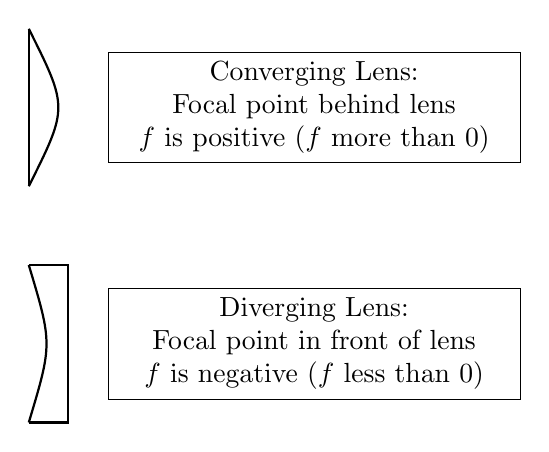
\begin{tikzpicture}
%\draw[step=1cm,gray,very thin] (-2,-2) grid (10,10);

\draw[thick](0,3) -- (0,5);
\draw[thick](0,3) .. controls (0.5,4) .. (0,5);

\node[draw, anchor=west, align=center, text width=5cm] at (1,4) {Converging Lens:\\ Focal point behind lens\\ $f$ is positive ($f$ more than 0)};

\draw[thick](0,0) -- (0.5,0) -- (0.5,2) -- (0,2);
\draw[thick](0,0) .. controls (0.3,1) .. (0,2);

\node[draw, anchor=west, align=center, text width=5cm] at (1,1) {Diverging Lens:\\ Focal point in front of lens\\ $f$ is negative ($f$ less than 0)};

\end{tikzpicture}
\columnbreak

\subsection{Sign convention}
\begin{center}
\begin{tabular}{ |c|c|c| } 
 \hline
  & Front of lens & Behind lens \\ 
  \hline
 f & Negative (-) & Positive (+) \\ 
 \hline
 p & Positive (+) & Negative (-) \\ 
 \hline
 q & Negative (-) & Positive (+) \\
 \hline
\end{tabular}
\end{center}
\end{multicols}

\subsection{Combining lenses}
\begin{center}
\small
\begin{tikzpicture}
%\draw[step=1cm,gray,very thin] (0,0) grid (14,6);

\draw[thick,->](1,3) -- (1,4);

\node[anchor=south, align=center] at (2.5,4) {$p_1$};

\draw[thick,<->](1,4) -- (4,4);

\filldraw (1,4) circle (2pt);

\draw[thick](4,1) rectangle (5,5);

\node[anchor=north, align=center] at (4.5,1) {$f_1$};

\draw[thick](10,1) rectangle (11,5);

\node[anchor=north, align=center] at (10.5,1) {$f_2$};

\draw[thick,<->](5,5) -- (10,5);

\node[anchor=south, align=center] at (7.5,5) {$d$};

\draw[thick,<->](11,4) -- (13,4);

\draw[thick,<->](5,2) -- (7,2);
\node[anchor=north, align=center] at (6,2) {$q_1$};
\draw[thick,<->](7,2) -- (10,2);
\node[anchor=north, align=center] at (8.5,2) {$p_2$};

\filldraw (13,4) circle (2pt);

\draw[thick,->](13,3) -- (13,4);

\node[anchor=south, align=center] at (12,4) {$q_2$};

\draw[thick,dashed](0,3) -- (14,3);

\end{tikzpicture}

\end{center}

\begin{multicols}{2}
{
%\begin{center}
\subsubsection{Working with multiple lenses}
\[
\boxed{\frac{1}{d-q_1}+\frac{1}{q_2}=\frac{1}{f_2}}
\]
%\end{center}
}

\columnbreak

%\begin{center}
\subsubsection{As $d\longrightarrow 0$}

\[
\boxed{\frac{1}{f_{\text{eff}}}=\frac{1}{f_1}+\frac{1}{f_2}}
\]

Two lenses stuck together ($d \approx 0$) may be treated as a single lens with a new effective focal length $f_{\text{eff}}$.
%\end{center}

\end{multicols}

\newpage

\section{Magnetism}

\subsection{Lorentz force law}

The force acting on a charged particle $q$ in an electric field $\vec{E}$ and magnetic field $\vec{B}$ and moving with velocity $\vec{v}$:

\[
\boxed{\vec{F} = q\left(\vec{E} + \vec{v} \times \vec{B}\right)}
\]

\subsection{Magnetic flux}

Magnetic flux through a wire loop of area $\vec{A}$ in a field $\vec{B}$ that is making an angle $\theta$ perpendicular to the loop, in units of weber:

\[
\boxed{
\phi_B = \int \vec{B} \cdot \mathrm{d}\vec{A}
}
\]

Simplifies when the magnetic field is constant over the area of the wire loop:

\[
\boxed{
\phi_B = \vec{B} \cdot \vec{A}
}
\]

\[
\boxed{
\phi_B = BA\cos(\theta)
}
\]

\subsubsection{Faraday's law}

Faraday's law states that electromotive force is inducted in a conductor when there is a change in the number of field lines passing through it, or when it cuts across field lines. The electromotive force $\varepsilon$ induced in a wire loop is the rate of change of flux through it.

\[
\boxed{
\varepsilon = -\frac{\mathrm{d}\phi_B}{\mathrm{d}t} = -\frac{\Delta \phi_B}{\Delta t}
}
\]

\subsubsection{Lenz's law}

Lenz's law states that induced current will appear in such a direction that it opposes the charge that produced it.

\subsubsection{Electromotive force in a coil}

Given a coil of $N$ turns:

\[
\boxed{
\varepsilon=-N\frac{\Delta \phi_B}{\Delta t}
}
\]

\newpage

\subsection{Magnetic induction from a current in a wire}

\subsubsection{Magnetic field at the centre of a coil}

Given a coil of $N$ turns, radius $r$ and carrying current $i$:

\[
\boxed{
B=\frac{\mu_0 Ni}{2r}
}
\]

\subsubsection{Magnetic field on the axis of a solenoid}

Given a solenoid of $N$ turns over an axial length $l$:

\[
\boxed{
B = \frac{\mu_0 Ni}{l}
}
\]

\subsubsection{Magnetic field from a straight wire}

At a distance $r$ from a wire carrying current $i$, with the position subtending angles $\theta_1$ and $\theta_2$ from the ends of the wire"

\[
\boxed{
B = \frac{\mu_0 i}{4\pi r}\left(\cos(\theta_1) + \cos(\theta_2)\right)
}
\]

\subsubsection{Magnetic field from an infinitely long wire}

Given that our wire is now infinitely long, meaning that $\theta_1 \longrightarrow 0$ and $\theta_2 \longrightarrow 0$:

\[
\boxed{
B = \frac{\mu_0 i}{2\pi r}
}
\]

\subsection{Cyclotron concepts}

\subsubsection{Radius of motion of a particle in a magnetic field}

Assuming that a field $B$ acts perpendicularly to the plane of orbit of a particle $q$ and mass $m$ moving with velocity $v$:

\[
\boxed{
r = \frac{mv}{qB}
}
\]\\

\begin{multicols}{2}

\subsubsection{Angular frequency}

\[
\boxed{
\omega = \frac{v}{r}=\frac{qB}{m}
}
\]

\columnbreak

\subsubsection{Cyclotron frequency}

\[
\boxed{
f = \frac{\omega}{2\pi}=\frac{qB}{2\pi m}
}
\]

\end{multicols}

\newpage

\section{Modern physics}

\subsection{Rapidity}

Given a a frame of reference that moves at a velocity $v$, and a variable $\beta$ defined as $\frac{v}{c}$, and where $\zeta$ is the rapidity:

\[
\boxed{
\tanh(\zeta) = \beta
}
\]

\subsubsection{Hyperbolic identities}

\[
\boxed{
\cosh(\zeta) = \frac{1}{\sqrt{1 - \beta^2}} = \frac{1}{\sqrt{1-\frac{v^2}{c^2}}}
}\text{ }
\boxed{
\sinh(\zeta) = \frac{\beta}{\sqrt{1 - \beta^2}} = \frac{\frac{v}{c}}{\sqrt{1-\frac{v^2}{c^2}}}
}\text{ }
\boxed{
\tanh(\zeta) = \frac{\sinh(\zeta)}{\cosh(\zeta)}
}
\]

\[
\boxed{
\cosh^2(\zeta) - \sinh^2(\zeta) = 1
}
\]

\subsection{Length contraction}

Given a speed $v$, and a proper length (at rest) of $L$:

\[
\boxed{
L'=\frac{L}{\cosh(\zeta)}=L\sqrt{1 - \beta^2} = L\sqrt{1 - \frac{v^2}{c^2}}
}
\]

\subsection{Time dilation}

Given a speed $v$, and a proper time (at rest) of $\Delta\tau$:

\[
\boxed{
\Delta\tau' = \Delta\tau\cosh(\zeta) = \frac{\Delta\tau}{\sqrt{1 - \beta^2}} = \frac{\Delta\tau}{\sqrt{1 - \frac{v^2}{c^2}}}
}
\]

\subsection{Mass dilation}

Given a rest mass $m$ and a frame moving at $v$:

\[
\boxed{
m' = m\cosh(\zeta) = \frac{m}{\sqrt{1 - \beta^2}} = \frac{m}{\sqrt{1 - \frac{v^2}{c^2}}}
}
\]

\subsection{Velocity addition}

Given an object moving at $v_0$ (rapidity $\zeta_0$) in a frame $S$, and a frame $S'$ moving at a speed $v$ (rapidity $\zeta$) relative to $S$, the speed ($v_0')$ and rapidity ($\zeta_0'$) in $S'$ can be found:

\[
\boxed{
\zeta_0' = \zeta_0 - \zeta
} \text{ or } 
\boxed{
v_0' = \frac{v_0 - v}{1 - \frac{v_0 v}{c^2}}
}
\]

\newpage

\subsection{Energy}

Given a particle of rest mass $m_0$ moving at $v_0$:

\[
\boxed{
\text{Total Energy } = E = m_0 c^2 \cosh(\zeta_0) = \frac{m_0 c^2}{\sqrt{1 - \beta^2}} = \frac{m_0 c^2}{\sqrt{1 - \frac{v_0^2}{c^2}}}
}
\]

\subsubsection{Energy at low speeds}

If $\left|\frac{v_0}{c}\right| << 1$, we can use a Taylor expansion like $(1 + x)^\alpha = 1 + \alpha x + O(x^2)$ to recover Newtonian kinetic energy:

\[
\boxed{
E = m_o c^2 + \frac{1}{2}m_0 v_0^2 + O\left(\frac{mv_0^4}{c^2}\right)
}
\]

The term $m_0 c^2$ is the rest energy, and $\frac{1}{2}m_0v_0^2$ is Newtonian kinetic energy.

\subsubsection{Energy in a different frame}

Given a frame of rapidity $\zeta_0$ and another frame of relative rapidity $\zeta$:

\[
\boxed{
E' = m_0 c^2 \cosh(\zeta_0 - \zeta) = m_0 c^2 \cosh(\zeta_0')}\text{ where } \zeta_0' = \zeta_0 - \zeta
\]

\subsection{Momentum}

Given a particle of rest mass $m_0$ moving at $v_0$:

\[
\boxed{
p = m_0 c \sinh(\zeta_0) = \frac{m_0 c \beta}{\sqrt{1 - \beta^2}} = \frac{m_0 v_0}{\sqrt{1 - \frac{v_0^2}{c^2}}}
}
\]

\subsubsection{Momentum at low speeds}

If $\left|\frac{v_0}{c}\right| << 1$, we can use a Taylor expansion like $(1 + x)^\alpha = 1 + \alpha x + O(x^2)$ to recover Newtonian momentum:

\[
\boxed{
p = m_0v_0 + O\left(\frac{mv_0^3}{c^2}\right)
}
\]

\subsubsection{Momentum in a different frame}

Given a frame of rapidity $\zeta_0$ and another frame of relative rapidity $\zeta$:

\[
\boxed{
p' = m_0 c \sinh(\zeta_0 - \zeta) = m_0 c \sinh(\zeta_0')}\text{ where } \zeta_0' = \zeta_0 - \zeta
\]

\newpage

\section{Thermodynamics}

\end{document}
